\documentclass{article}

\usepackage{amsmath,amssymb,amsthm,float}

\setlength{\oddsidemargin}{0.25 in}
\setlength{\evensidemargin}{-0.25 in}
\setlength{\topmargin}{-0.6 in}
\setlength{\textwidth}{6.5 in}
\setlength{\textheight}{8.5 in}
\setlength{\headsep}{0.75 in}
\setlength{\parindent}{0 in}
\setlength{\parskip}{0.1 in}

\newtheorem{theorem}{Theorem}
\newtheorem{corollary}{Corollary}
\newtheorem{proposition}{Proposition}
\newtheorem*{remark}{Remark}
\theoremstyle{definition}
\newtheorem{example}{Example}
\newtheorem{definition}{Definition}

\newcommand{\lecture}[4]{
   \pagestyle{myheadings}
   \thispagestyle{plain}
   \newpage
%   \setcounter{lecnum}{#1}
   \setcounter{page}{1}
   \noindent
   \begin{center}
   \framebox{
      \vbox{\vspace{2mm}
    \hbox to 6.58in { {\bf CSC~565: Graph Theory
                        \hfill North Carolina State University} }
    \hbox to 6.58in { {\bf Fall 2019
                        \hfill Computer Science} }
       \vspace{4mm}
       \hbox to 6.28in { {\Large \hfill Lecture #1: #2  \hfill} }
       \vspace{2mm}
       \hbox to 6.28in { {\it Lecturer: {\it Don Sheehy {\tt <drsheehy@ncsu.edu>}} \hfill Scribe: #4} }
      \vspace{2mm}}
   }
   \end{center}
   \markboth{Lecture #1: #2}{Lecture #1: #2}
   \vspace*{4mm}
}

\usepackage{graphics,tikz}
\def\geom{\text{geom}}
\def\sim{\text{sim}}
\def\R{\mathbb{R}}\begin{document}

%FILL IN THE RIGHT INFO.
%\lecture{**LECTURE-NUMBER**}{**DATE**}{**LECTURER**}{**SCRIBE**}
\lecture{8}{Sep 18, 2019}{Don Sheehy}{Palash Gupta, Rishabh Agrawal, Jash Dhakad }

  % \title{Lecture 6}
  % \author{Scribed by: }
  % \maketitle
\section{Handshake Lemma}
\begin{definition}
The number of vertices of odd degree in the graph is even.\\

\begin{equation*}
\sum\nolimits_{v \in V_G} deg(v) = 2 | E_G|
\end{equation*}

\end{definition}

\section{Tree}
\begin{theorem}
  Prove that every tree can be drawn in a plane $\R^2$  without crossing.
  \end{theorem}
      \begin{proof}
 To prove this we'll give an algorithm to draw the tree. Consider a given tree $G$ and select any arbitrary point. Consider it to be the root. Now label all the points by the distance from the root. For example the label of root would be 0. As it is a tree,it is connected and all vertices will have a label. Place all the vertices with the same label in the same horizontal level such that if a vertex $p$ comes before vertex $q$ in a horizontal level, then the children of vertex $p$ will come before the children of $q$ in the next horizontal level. We start with the root at the top. This algorithm is illustrated in the Figure \ref{fig:treeDrawing} and \ref{fig:multiLevelTree}.

Let us assume that there is a crossing between the edges of a tree. Let $(p,q)$ and $(r,s)$ be two such edges, where $p$ is the parent of $q$ and $r$ is the parent of $s$. Level of $p$ and $r$ has to be the same because if they were on the different levels edges are vertically separated and cannot intersect. Let $p$ and $r$ be at the level $l$ and $s$ and $q$ at level $l+1$. In order for the crossing to occur, the following condition should be met. If ($p$ is before $r$) then ($s$ is before $q$). This is shown in Figure. \ref{fig:edgeCrossing}. But as stated above if $p$ is before $r$, then all children of $p$ should be placed before all children of $r$. This would mean that $q$ should be placed before s. That would mean the aforementioned condition cannot be satisfied and edge crossing cannot occur.
          \begin{figure}[H]
\begin{center}

    \tikzset{every picture/.style={line width=0.75pt}} %set default line width to 0.75pt        
    
    \begin{tikzpicture}[x=0.75pt,y=0.75pt,yscale=-1,xscale=1]
    %uncomment if require: \path (0,443.8833312988281); %set diagram left start at 0, and has height of 443.8833312988281
    
    %Shape: Ellipse [id:dp013251641491293431] 
    \draw   (308.25,53.5) .. controls (308.25,44.39) and (315.61,37) .. (324.69,37) .. controls (333.77,37) and (341.13,44.39) .. (341.13,53.5) .. controls (341.13,62.62) and (333.77,70.01) .. (324.69,70.01) .. controls (315.61,70.01) and (308.25,62.62) .. (308.25,53.5) -- cycle ;
    %Shape: Ellipse [id:dp3504718800593517] 
    \draw   (141.13,140.36) .. controls (141.13,131.24) and (148.49,123.85) .. (157.57,123.85) .. controls (166.65,123.85) and (174.02,131.24) .. (174.02,140.36) .. controls (174.02,149.47) and (166.65,156.86) .. (157.57,156.86) .. controls (148.49,156.86) and (141.13,149.47) .. (141.13,140.36) -- cycle ;
    %Shape: Ellipse [id:dp6770703678032634] 
    \draw   (312.49,140.36) .. controls (312.49,131.24) and (319.85,123.85) .. (328.93,123.85) .. controls (338.01,123.85) and (345.38,131.24) .. (345.38,140.36) .. controls (345.38,149.47) and (338.01,156.86) .. (328.93,156.86) .. controls (319.85,156.86) and (312.49,149.47) .. (312.49,140.36) -- cycle ;
    %Shape: Ellipse [id:dp9905805112353976] 
    \draw   (476.22,142.06) .. controls (476.22,132.94) and (483.58,125.55) .. (492.66,125.55) .. controls (501.74,125.55) and (509.1,132.94) .. (509.1,142.06) .. controls (509.1,151.17) and (501.74,158.56) .. (492.66,158.56) .. controls (483.58,158.56) and (476.22,151.17) .. (476.22,142.06) -- cycle ;
    %Shape: Ellipse [id:dp7511891788503602] 
    \draw   (92.77,257.86) .. controls (92.77,248.75) and (100.14,241.36) .. (109.22,241.36) .. controls (118.3,241.36) and (125.66,248.75) .. (125.66,257.86) .. controls (125.66,266.98) and (118.3,274.37) .. (109.22,274.37) .. controls (100.14,274.37) and (92.77,266.98) .. (92.77,257.86) -- cycle ;
    %Shape: Ellipse [id:dp4929165659224152] 
    \draw   (247.17,261.27) .. controls (247.17,252.15) and (254.53,244.76) .. (263.61,244.76) .. controls (272.69,244.76) and (280.06,252.15) .. (280.06,261.27) .. controls (280.06,270.38) and (272.69,277.77) .. (263.61,277.77) .. controls (254.53,277.77) and (247.17,270.38) .. (247.17,261.27) -- cycle ;
    %Shape: Ellipse [id:dp8063605361374856] 
    \draw   (362.54,263.06) .. controls (362.54,253.52) and (370.24,245.78) .. (379.75,245.78) .. controls (389.25,245.78) and (396.95,253.52) .. (396.95,263.06) .. controls (396.95,272.59) and (389.25,280.33) .. (379.75,280.33) .. controls (370.24,280.33) and (362.54,272.59) .. (362.54,263.06) -- cycle ;
    %Shape: Ellipse [id:dp8337477650523604] 
    \draw   (440.37,259.73) .. controls (440.37,250.62) and (447.74,243.23) .. (456.82,243.23) .. controls (465.9,243.23) and (473.26,250.62) .. (473.26,259.73) .. controls (473.26,268.85) and (465.9,276.24) .. (456.82,276.24) .. controls (447.74,276.24) and (440.37,268.85) .. (440.37,259.73) -- cycle ;
    %Shape: Ellipse [id:dp3928775345004998] 
    \draw   (537.93,261.44) .. controls (537.93,252.32) and (545.29,244.93) .. (554.37,244.93) .. controls (563.46,244.93) and (570.82,252.32) .. (570.82,261.44) .. controls (570.82,270.55) and (563.46,277.94) .. (554.37,277.94) .. controls (545.29,277.94) and (537.93,270.55) .. (537.93,261.44) -- cycle ;
    %Shape: Ellipse [id:dp9093116826516576] 
    \draw   (70.72,357.49) .. controls (70.72,348.37) and (78.08,340.98) .. (87.16,340.98) .. controls (96.24,340.98) and (103.6,348.37) .. (103.6,357.49) .. controls (103.6,366.6) and (96.24,373.99) .. (87.16,373.99) .. controls (78.08,373.99) and (70.72,366.6) .. (70.72,357.49) -- cycle ;
    %Shape: Ellipse [id:dp27902713029120785] 
    \draw   (152.16,357.49) .. controls (152.16,348.37) and (159.52,340.98) .. (168.6,340.98) .. controls (177.68,340.98) and (185.04,348.37) .. (185.04,357.49) .. controls (185.04,366.6) and (177.68,373.99) .. (168.6,373.99) .. controls (159.52,373.99) and (152.16,366.6) .. (152.16,357.49) -- cycle ;
    %Straight Lines [id:da04357009839396775] 
    \draw    (167.36,128.07) -- (313.73,66.6) ;
    
    
    %Straight Lines [id:da8061802219685432] 
    \draw    (324.69,70.01) -- (328.93,123.85) ;
    
    
    %Straight Lines [id:da3655604140104268] 
    \draw    (337.74,61.65) -- (478.28,132.65) ;
    
    
    %Straight Lines [id:da5805838548261475] 
    \draw    (157.57,156.86) -- (109.22,241.36) ;
    
    
    %Straight Lines [id:da9054176909146017] 
    \draw    (263.61,244.76) -- (328.93,156.86) ;
    
    
    %Straight Lines [id:da9061864638958759] 
    \draw    (328.93,156.86) -- (379.75,245.78) ;
    
    
    %Straight Lines [id:da8044378455305757] 
    \draw    (456.82,243.23) -- (492.66,158.56) ;
    
    
    %Straight Lines [id:da20170981607224014] 
    \draw    (492.66,158.56) -- (554.37,244.93) ;
    
    
    %Straight Lines [id:da5584656407111704] 
    \draw    (109.22,274.37) -- (87.16,340.98) ;
    
    
    %Straight Lines [id:da7963986274475852] 
    \draw    (109.22,274.37) -- (168.6,340.98) ;
    
    
    %Shape: Rectangle [id:dp6756680224361427] 
    \draw   (129.69,112.48) -- (533.49,112.48) -- (533.49,180.46) -- (129.69,180.46) -- cycle ;
    %Shape: Rectangle [id:dp6176081630971761] 
    \draw   (77.09,227.44) -- (604.75,227.44) -- (604.75,291.3) -- (77.09,291.3) -- cycle ;
    %Shape: Rectangle [id:dp25213388159487515] 
    \draw   (61.5,333.87) -- (208.58,333.87) -- (208.58,379) -- (61.5,379) -- cycle ;
    
    % Text Node
    \draw (358.1,51.04) node  [align=left] {root};
    
    
    \end{tikzpicture}
 \end{center}
 \caption{Tree drawing algorithm illustration}
 \label{fig:treeDrawing}
 \end{figure}

 \begin{figure}[H]
\begin{center}

    \tikzset{every picture/.style={line width=0.75pt}} %set default line width to 0.75pt        
    
    \begin{tikzpicture}[x=0.75pt,y=0.75pt,yscale=-1,xscale=1]
    %uncomment if require: \path (0,644); %set diagram left start at 0, and has height of 644
    
    %Straight Lines [id:da8679641386299183] 
    \draw    (129.1,48.12) -- (487.5,47) ;
    
    
    %Straight Lines [id:da1823278074000242] 
    \draw    (126.38,217.31) -- (484.78,216.19) ;
    
    
    %Straight Lines [id:da9237788777438267] 
    \draw    (115.5,132.72) -- (473.9,131.59) ;
    
    
    %Straight Lines [id:da15452186287705083] 
    \draw    (126.38,327.29) -- (484.78,326.16) ;
    
    
    %Shape: Ellipse [id:dp8451771890920043] 
    \draw   (304.17,47.56) .. controls (304.17,45.2) and (306.02,43.28) .. (308.3,43.28) .. controls (310.58,43.28) and (312.42,45.2) .. (312.42,47.56) .. controls (312.42,49.92) and (310.58,51.84) .. (308.3,51.84) .. controls (306.02,51.84) and (304.17,49.92) .. (304.17,47.56) -- cycle ;
    %Shape: Ellipse [id:dp3605618900924389] 
    \draw   (207.59,129.34) .. controls (207.59,126.97) and (209.44,125.06) .. (211.72,125.06) .. controls (214,125.06) and (215.84,126.97) .. (215.84,129.34) .. controls (215.84,131.7) and (214,133.61) .. (211.72,133.61) .. controls (209.44,133.61) and (207.59,131.7) .. (207.59,129.34) -- cycle ;
    %Shape: Ellipse [id:dp011738830314276583] 
    \draw   (251.1,213.93) .. controls (251.1,211.57) and (252.95,209.65) .. (255.23,209.65) .. controls (257.5,209.65) and (259.35,211.57) .. (259.35,213.93) .. controls (259.35,216.29) and (257.5,218.21) .. (255.23,218.21) .. controls (252.95,218.21) and (251.1,216.29) .. (251.1,213.93) -- cycle ;
    %Shape: Ellipse [id:dp016990569351802765] 
    \draw   (335.4,213.93) .. controls (335.4,211.57) and (337.25,209.65) .. (339.52,209.65) .. controls (341.8,209.65) and (343.65,211.57) .. (343.65,213.93) .. controls (343.65,216.29) and (341.8,218.21) .. (339.52,218.21) .. controls (337.25,218.21) and (335.4,216.29) .. (335.4,213.93) -- cycle ;
    %Shape: Ellipse [id:dp05248132494427582] 
    \draw   (419.7,213.93) .. controls (419.7,211.57) and (421.55,209.65) .. (423.82,209.65) .. controls (426.1,209.65) and (427.95,211.57) .. (427.95,213.93) .. controls (427.95,216.29) and (426.1,218.21) .. (423.82,218.21) .. controls (421.55,218.21) and (419.7,216.29) .. (419.7,213.93) -- cycle ;
    %Shape: Ellipse [id:dp4618941899395681] 
    \draw   (444.17,326.72) .. controls (444.17,324.36) and (446.02,322.45) .. (448.3,322.45) .. controls (450.57,322.45) and (452.42,324.36) .. (452.42,326.72) .. controls (452.42,329.09) and (450.57,331) .. (448.3,331) .. controls (446.02,331) and (444.17,329.09) .. (444.17,326.72) -- cycle ;
    %Shape: Ellipse [id:dp48843211369986905] 
    \draw   (452.33,213.93) .. controls (452.33,211.57) and (454.18,209.65) .. (456.45,209.65) .. controls (458.73,209.65) and (460.58,211.57) .. (460.58,213.93) .. controls (460.58,216.29) and (458.73,218.21) .. (456.45,218.21) .. controls (454.18,218.21) and (452.33,216.29) .. (452.33,213.93) -- cycle ;
    %Shape: Ellipse [id:dp5262182698248602] 
    \draw   (310.93,129.34) .. controls (310.93,126.97) and (312.77,125.06) .. (315.05,125.06) .. controls (317.33,125.06) and (319.18,126.97) .. (319.18,129.34) .. controls (319.18,131.7) and (317.33,133.61) .. (315.05,133.61) .. controls (312.77,133.61) and (310.93,131.7) .. (310.93,129.34) -- cycle ;
    %Shape: Ellipse [id:dp60762823657962] 
    \draw   (408.82,326.72) .. controls (408.82,324.36) and (410.67,322.45) .. (412.95,322.45) .. controls (415.22,322.45) and (417.07,324.36) .. (417.07,326.72) .. controls (417.07,329.09) and (415.22,331) .. (412.95,331) .. controls (410.67,331) and (408.82,329.09) .. (408.82,326.72) -- cycle ;
    %Shape: Ellipse [id:dp005588247345829078] 
    \draw   (381.63,213.93) .. controls (381.63,211.57) and (383.48,209.65) .. (385.75,209.65) .. controls (388.03,209.65) and (389.88,211.57) .. (389.88,213.93) .. controls (389.88,216.29) and (388.03,218.21) .. (385.75,218.21) .. controls (383.48,218.21) and (381.63,216.29) .. (381.63,213.93) -- cycle ;
    %Shape: Ellipse [id:dp8196914442684315] 
    \draw   (411.54,129.34) .. controls (411.54,126.97) and (413.39,125.06) .. (415.67,125.06) .. controls (417.94,125.06) and (419.79,126.97) .. (419.79,129.34) .. controls (419.79,131.7) and (417.94,133.61) .. (415.67,133.61) .. controls (413.39,133.61) and (411.54,131.7) .. (411.54,129.34) -- cycle ;
    %Shape: Ellipse [id:dp6919024995083671] 
    \draw   (305.58,326.72) .. controls (305.58,324.36) and (307.43,322.45) .. (309.7,322.45) .. controls (311.98,322.45) and (313.83,324.36) .. (313.83,326.72) .. controls (313.83,329.09) and (311.98,331) .. (309.7,331) .. controls (307.43,331) and (305.58,329.09) .. (305.58,326.72) -- cycle ;
    %Shape: Ellipse [id:dp9396365309919391] 
    \draw   (359.87,326.72) .. controls (359.87,324.36) and (361.72,322.45) .. (364,322.45) .. controls (366.28,322.45) and (368.12,324.36) .. (368.12,326.72) .. controls (368.12,329.09) and (366.28,331) .. (364,331) .. controls (361.72,331) and (359.87,329.09) .. (359.87,326.72) -- cycle ;
    %Shape: Ellipse [id:dp009053637437229534] 
    \draw   (476.53,326.16) .. controls (476.53,323.8) and (478.38,321.88) .. (480.66,321.88) .. controls (482.93,321.88) and (484.78,323.8) .. (484.78,326.16) .. controls (484.78,328.52) and (482.93,330.44) .. (480.66,330.44) .. controls (478.38,330.44) and (476.53,328.52) .. (476.53,326.16) -- cycle ;
    %Straight Lines [id:da44184321284323913] 
    \draw    (308.3,51.84) -- (215.84,129.34) ;
    
    
    %Straight Lines [id:da21669874790911836] 
    \draw    (308.3,51.84) -- (315.05,129.34) ;
    
    
    %Straight Lines [id:da45537103314486427] 
    \draw    (308.3,47.56) -- (415.67,129.34) ;
    
    
    %Straight Lines [id:da44156620034838145] 
    \draw    (211.72,129.34) -- (255.23,213.93) ;
    
    
    %Straight Lines [id:da24037049620640927] 
    \draw    (315.05,129.34) -- (339.52,213.93) ;
    
    
    %Straight Lines [id:da0302570993886776] 
    \draw    (415.67,129.34) -- (385.75,213.93) ;
    
    
    %Straight Lines [id:da6370870438774625] 
    \draw    (415.67,129.34) -- (423.82,213.93) ;
    
    
    %Straight Lines [id:da10986501157735229] 
    \draw    (415.67,129.34) -- (456.45,213.93) ;
    
    
    %Straight Lines [id:da8402963105985113] 
    \draw    (423.82,213.93) -- (480.66,326.16) ;
    
    
    %Straight Lines [id:da7833025415255381] 
    \draw    (423.82,218.21) -- (412.95,326.72) ;
    
    
    %Straight Lines [id:da9340919497733094] 
    \draw    (423.82,218.21) -- (448.3,326.72) ;
    
    
    %Straight Lines [id:da0344499106711873] 
    \draw    (385.75,213.93) -- (359.87,326.72) ;
    
    
    %Straight Lines [id:da6165594303193094] 
    \draw    (339.52,213.93) -- (309.7,326.72) ;
    
    
    
    
    
    
    \end{tikzpicture}
\end{center}
\caption{Drawing multi level tree}
\label{fig:multiLevelTree}
\end{figure}

\begin{figure}[H]

\begin{center}
    
    \tikzset{every picture/.style={line width=0.75pt}} %set default line width to 0.75pt        
    
    \begin{tikzpicture}[x=0.75pt,y=0.75pt,yscale=-1,xscale=1]
    %uncomment if require: \path (0,563); %set diagram left start at 0, and has height of 563
    
    %Straight Lines [id:da34524389152258017] 
    \draw    (257,112) -- (384.5,233) ;
    
    
    %Straight Lines [id:da15616149174393135] 
    \draw    (391,110) -- (254.5,235) ;
    
    
    
    % Text Node
    \draw (247,105) node  [align=left] {p};
    % Text Node
    \draw (243,244) node  [align=left] {s};
    % Text Node
    \draw (408,101) node  [align=left] {r};
    % Text Node
    \draw (396,240) node  [align=left] {q};
    \end{tikzpicture}
\end{center}
\caption{Edge crossing}
\label{fig:edgeCrossing}
\end{figure}
\end{proof}
  
\begin{theorem}
Every binary tree has at least one edge (u,v) such that G \textbackslash(u,v) has 2 components and neither has more than \{(2n)/3 + 1\} vertices.
\end{theorem}

\begin{proof}[Proof idea]
    This can be proved by moving down the tree such that if the number of vertices in a given subtree is greater than $2n/3$, we move to the child. There will come a point, where both the children have less than or equal to $2n/3$ sized subtrees. We remove the edge with the child from this node.


%\begin{figure}
%\begin{center}
%\tikzset{every picture/.style={line width=0.75pt}} %set default line width to 0.75pt        
%
%    \begin{tikzpicture}[x=0.75pt,y=0.75pt,yscale=-1,xscale=1]
%    %uncomment if require: \path (0,300); %set diagram left start at 0, and has height of 300
%    
%    %Shape: Ellipse [id:dp5026941740532689] 
%    \draw   (263.97,36.47) .. controls (263.97,32.41) and (268.66,29.12) .. (274.45,29.12) .. controls (280.23,29.12) and (284.92,32.41) .. (284.92,36.47) .. controls (284.92,40.52) and (280.23,43.81) .. (274.45,43.81) .. controls (268.66,43.81) and (263.97,40.52) .. (263.97,36.47) -- cycle ;
%    %Shape: Ellipse [id:dp8052290539693855] 
%    \draw   (248.82,108.6) .. controls (248.82,104.55) and (253.52,101.25) .. (259.3,101.25) .. controls (265.09,101.25) and (269.78,104.55) .. (269.78,108.6) .. controls (269.78,112.66) and (265.09,115.95) .. (259.3,115.95) .. controls (253.52,115.95) and (248.82,112.66) .. (248.82,108.6) -- cycle ;
%    %Shape: Ellipse [id:dp5260936609004553] 
%    \draw   (158.75,106.93) .. controls (158.75,102.87) and (163.44,99.58) .. (169.23,99.58) .. controls (175.01,99.58) and (179.7,102.87) .. (179.7,106.93) .. controls (179.7,110.98) and (175.01,114.28) .. (169.23,114.28) .. controls (163.44,114.28) and (158.75,110.98) .. (158.75,106.93) -- cycle ;
%    %Shape: Ellipse [id:dp0005502308215511453] 
%    \draw   (302.23,66.1) .. controls (302.23,62.05) and (306.92,58.75) .. (312.71,58.75) .. controls (318.49,58.75) and (323.18,62.05) .. (323.18,66.1) .. controls (323.18,70.16) and (318.49,73.45) .. (312.71,73.45) .. controls (306.92,73.45) and (302.23,70.16) .. (302.23,66.1) -- cycle ;
%    %Shape: Ellipse [id:dp49902676693437586] 
%    \draw   (209.77,65.54) .. controls (209.77,61.49) and (214.46,58.2) .. (220.24,58.2) .. controls (226.03,58.2) and (230.72,61.49) .. (230.72,65.54) .. controls (230.72,69.6) and (226.03,72.89) .. (220.24,72.89) .. controls (214.46,72.89) and (209.77,69.6) .. (209.77,65.54) -- cycle ;
%    %Straight Lines [id:da189102538082779] 
%    \draw    (274.45,43.81) -- (220.24,58.2) ;
%    
%    
%    %Straight Lines [id:da8842093294465067] 
%    \draw    (274.45,43.81) -- (312.71,58.75) ;
%    
%    
%    %Straight Lines [id:da3777940096483836] 
%    \draw    (169.23,99.58) -- (220.24,72.89) ;
%    
%    
%    %Straight Lines [id:da8028300693428679] 
%    \draw    (259.3,101.25) -- (220.24,72.89) ;
%    
%    
%    %Shape: Ellipse [id:dp65926601971189] 
%    \draw   (191.97,232.47) .. controls (191.97,228.41) and (196.66,225.12) .. (202.45,225.12) .. controls (208.23,225.12) and (212.92,228.41) .. (212.92,232.47) .. controls (212.92,236.52) and (208.23,239.81) .. (202.45,239.81) .. controls (196.66,239.81) and (191.97,236.52) .. (191.97,232.47) -- cycle ;
%    %Shape: Ellipse [id:dp6411355252121014] 
%    \draw   (109.97,231.47) .. controls (109.97,227.41) and (114.66,224.12) .. (120.45,224.12) .. controls (126.23,224.12) and (130.92,227.41) .. (130.92,231.47) .. controls (130.92,235.52) and (126.23,238.81) .. (120.45,238.81) .. controls (114.66,238.81) and (109.97,235.52) .. (109.97,231.47) -- cycle ;
%    %Straight Lines [id:da5016048102790736] 
%    \draw    (165.12,193.65) -- (153.12,202.65) ;
%    
%    
%    %Straight Lines [id:da9396382704817337] 
%    \draw    (148.12,205.65) -- (136.12,214.65) ;
%    
%    
%    %Straight Lines [id:da5266599741439887] 
%    \draw    (132.45,215.12) -- (120.45,224.12) ;
%    
%    
%    %Straight Lines [id:da8645457315504854] 
%    \draw    (169.22,196.65) -- (183.22,208.65) ;
%    
%    
%    %Straight Lines [id:da5660632425660811] 
%    \draw    (187.22,212.65) -- (202.45,225.12) ;
%    
%    
%    %Shape: Circle [id:dp8947826209460452] 
%    \draw   (377.52,234.87) .. controls (377.52,229.48) and (381.89,225.1) .. (387.29,225.1) .. controls (392.69,225.1) and (397.07,229.48) .. (397.07,234.87) .. controls (397.07,240.27) and (392.69,244.65) .. (387.29,244.65) .. controls (381.89,244.65) and (377.52,240.27) .. (377.52,234.87) -- cycle ;
%    %Shape: Circle [id:dp7757098827760354] 
%    \draw   (415.52,284.87) .. controls (415.52,279.48) and (419.89,275.1) .. (425.29,275.1) .. controls (430.69,275.1) and (435.07,279.48) .. (435.07,284.87) .. controls (435.07,290.27) and (430.69,294.65) .. (425.29,294.65) .. controls (419.89,294.65) and (415.52,290.27) .. (415.52,284.87) -- cycle ;
%    %Shape: Circle [id:dp5978185823414772] 
%    \draw   (329.52,284.87) .. controls (329.52,279.48) and (333.89,275.1) .. (339.29,275.1) .. controls (344.69,275.1) and (349.07,279.48) .. (349.07,284.87) .. controls (349.07,290.27) and (344.69,294.65) .. (339.29,294.65) .. controls (333.89,294.65) and (329.52,290.27) .. (329.52,284.87) -- cycle ;
%    %Straight Lines [id:da544800641882542] 
%    \draw    (387.29,244.65) -- (339.29,275.1) ;
%    
%    
%    %Straight Lines [id:da0421722164760574] 
%    \draw    (387.29,244.65) -- (425.29,275.1) ;
%    
%    
%    
%    % Text Node
%    \draw (274.45,36.47) node  [align=left] {n};
%    % Text Node
%    \draw (220.24,65.54) node  [align=left] {?};
%    % Text Node
%    \draw (312.71,66.1) node  [align=left] {?};
%    % Text Node
%    \draw (169.23,106.93) node  [align=left] {?};
%    % Text Node
%    \draw (259.3,108.6) node  [align=left] {?};
%    % Text Node
%    \draw (170.14,146.17) node  [align=left] {..\\...\\\\..\\..};
%    % Text Node
%    \draw (120.45,231.47) node  [align=left] {1};
%    % Text Node
%    \draw (202.45,232.47) node  [align=left] {1};
%    % Text Node
%    \draw (283.13,232.93) node  [align=left] {else somewhere };
%    % Text Node
%    \draw (419.07,234.1) node  [align=left] {$>2n/3$};
%    % Text Node
%    \draw (303.03,285.17) node  [align=left] {$< n/3$};
%    % Text Node
%    \draw (459.03,285) node  [align=left] {$< n/3$};
%    
%    
%    \end{tikzpicture}
%\end{center}
%\end{figure}
\end{proof}


\section{Outer Planar Graph}
\begin{definition}
A graph is outer planar if it can be embedded in the plane so that every vertex is on the same face.

${G \rightarrow geom (G) \subseteq {\R^n} \xrightarrow[\text{}]{\text{embed}} Embedding  \subseteq {\R^2}}$

The second mapping (the embed one) is an injective mapping.

\end{definition}


\begin{definition}
Faces of $\underbar{G}$ are path connected components of ${\R^2}$\textbackslash\underbar{G} 
\end{definition}

\begin{definition}
    Vertices on the same face means, they can be connected using a path which is only composed of points of one face.
\end{definition}

\begin{theorem}
    $G$ is outer planar, iff it has no $K_{4}$ or $K_{2,3}$ minors
\end{theorem}

\begin{theorem}
    Any graph property expressed as forbidden minors is preserved by edge contractions.
\end{theorem}

\begin{proof}
    If a graph $M$ is not a minor of graph $G$, it cannot be the minor of $G'$ obtained by contracting the edges of graph $G$. This is because if $M$ was the minor of $G'$, it could be obtained by contracting $G'$, then it could also be obtained from $G$ by first contracting to $G'$ and then $M$. That would make it a minor of $G$.
\end{proof}

\begin{figure}[H]
    \begin{center}



\tikzset{every picture/.style={line width=0.75pt}} %set default line width to 0.75pt        

\begin{tikzpicture}[x=0.75pt,y=0.75pt,yscale=-1,xscale=1]
%uncomment if require: \path (0,300); %set diagram left start at 0, and has height of 300


% Text Node
\draw (120,128) node  [align=left] {G};
% Text Node
\draw (224,147) node  [align=left] {M};
% Text Node
\draw (158,174) node  [align=left] {G`};
% Text Node
\draw (87,157) node  [align=left] {Contraction};
% Connection
\draw    (130,129.83) -- (207.5,143.99) ;
\draw [shift={(207.5,143.99)}, rotate = 55.35] [color={rgb, 255:red, 0; green, 0; blue, 0 }  ][line width=0.75]    (-5.59,0) -- (5.59,0)(0,5.59) -- (0,-5.59)   ;

% Connection
\draw    (170.5,168.89) -- (207.5,153.75) ;
\draw [shift={(207.5,153.75)}, rotate = 382.75] [color={rgb, 255:red, 0; green, 0; blue, 0 }  ][line width=0.75]    (-5.59,0) -- (5.59,0)(0,5.59) -- (0,-5.59)   ;

% Connection
\draw    (129.09,139) -- (147.64,161.46) ;
\draw [shift={(148.91,163)}, rotate = 230.44] [color={rgb, 255:red, 0; green, 0; blue, 0 }  ][line width=0.75]    (10.93,-3.29) .. controls (6.95,-1.4) and (3.31,-0.3) .. (0,0) .. controls (3.31,0.3) and (6.95,1.4) .. (10.93,3.29)   ;


\end{tikzpicture}
\end{center}
\caption{Minors are invariants in edge contraction}
\end{figure}

\begin{corollary}
If a Graph G does not have a minor M, then its contraction G' also does not have a minor.
\end{corollary}


\begin{figure}[h!]
\label{fig:faces}
\begin{center}
    
    \tikzset{every picture/.style={line width=0.75pt}} %set default line width to 0.75pt        
    
    \begin{tikzpicture}[x=0.75pt,y=0.75pt,yscale=-1,xscale=1]
    %uncomment if require: \path (0,300); %set diagram left start at 0, and has height of 300
    
    %Flowchart: Decision [id:dp8888176421485359] 
    \draw   (199.56,94.7) -- (273.21,141.58) -- (199.56,188.46) -- (125.9,141.58) -- cycle ;
    %Shape: Ellipse [id:dp6760978318532891] 
    \draw   (198.47,95.91) .. controls (198.47,95.24) and (198.96,94.7) .. (199.56,94.7) .. controls (200.16,94.7) and (200.64,95.24) .. (200.64,95.91) .. controls (200.64,96.58) and (200.16,97.12) .. (199.56,97.12) .. controls (198.96,97.12) and (198.47,96.58) .. (198.47,95.91) -- cycle ;
    %Shape: Ellipse [id:dp2329693039703622] 
    \draw   (197.38,188.46) .. controls (197.38,187.79) and (197.87,187.24) .. (198.47,187.24) .. controls (199.07,187.24) and (199.56,187.79) .. (199.56,188.46) .. controls (199.56,189.12) and (199.07,189.67) .. (198.47,189.67) .. controls (197.87,189.67) and (197.38,189.12) .. (197.38,188.46) -- cycle ;
    %Shape: Ellipse [id:dp81170310784359] 
    \draw   (272.13,140.37) .. controls (272.13,139.7) and (272.61,139.16) .. (273.21,139.16) .. controls (273.81,139.16) and (274.3,139.7) .. (274.3,140.37) .. controls (274.3,141.04) and (273.81,141.58) .. (273.21,141.58) .. controls (272.61,141.58) and (272.13,141.04) .. (272.13,140.37) -- cycle ;
    %Shape: Ellipse [id:dp6595798796647364] 
    \draw   (125.9,141.58) .. controls (125.9,140.91) and (126.39,140.37) .. (126.99,140.37) .. controls (127.59,140.37) and (128.07,140.91) .. (128.07,141.58) .. controls (128.07,142.25) and (127.59,142.79) .. (126.99,142.79) .. controls (126.39,142.79) and (125.9,142.25) .. (125.9,141.58) -- cycle ;
    
    % Text Node
    \draw (322,138.32) node  [align=left] {};
    % Text Node
    \draw (120,180.32) node   {$$};
    
    
    \end{tikzpicture}
    \caption{Example to show faces}
\end{center}

\end{figure}
     
    
\begin{figure}[h!]
\begin{center}
    \tikzset{every picture/.style={line width=0.75pt}} %set default line width to 0.75pt        
    
    \begin{tikzpicture}[x=0.75pt,y=0.75pt,yscale=-1,xscale=1]
    %uncomment if require: \path (0,300); %set diagram left start at 0, and has height of 300
    
    %Shape: Ellipse [id:dp13065196607854535] 
    \draw   (186.38,164.26) .. controls (186.38,123.21) and (224.66,89.92) .. (271.88,89.92) .. controls (319.1,89.92) and (357.38,123.21) .. (357.38,164.26) .. controls (357.38,205.32) and (319.1,238.6) .. (271.88,238.6) .. controls (224.66,238.6) and (186.38,205.32) .. (186.38,164.26) -- cycle ;
    %Shape: Ellipse [id:dp803169309486954] 
    \draw   (268.06,89.92) .. controls (268.06,88.09) and (269.77,86.6) .. (271.88,86.6) .. controls (273.99,86.6) and (275.71,88.09) .. (275.71,89.92) .. controls (275.71,91.76) and (273.99,93.25) .. (271.88,93.25) .. controls (269.77,93.25) and (268.06,91.76) .. (268.06,89.92) -- cycle ;
    %Shape: Ellipse [id:dp7844010278319313] 
    \draw   (268.06,160.94) .. controls (268.06,159.1) and (269.77,157.62) .. (271.88,157.62) .. controls (273.99,157.62) and (275.71,159.1) .. (275.71,160.94) .. controls (275.71,162.77) and (273.99,164.26) .. (271.88,164.26) .. controls (269.77,164.26) and (268.06,162.77) .. (268.06,160.94) -- cycle ;
    %Shape: Ellipse [id:dp9725021620461569] 
    \draw   (335.6,208.74) .. controls (335.6,206.9) and (337.31,205.41) .. (339.42,205.41) .. controls (341.54,205.41) and (343.25,206.9) .. (343.25,208.74) .. controls (343.25,210.57) and (341.54,212.06) .. (339.42,212.06) .. controls (337.31,212.06) and (335.6,210.57) .. (335.6,208.74) -- cycle ;
    %Shape: Ellipse [id:dp8074058938003839] 
    \draw   (200.52,210.1) .. controls (200.52,208.27) and (202.23,206.78) .. (204.34,206.78) .. controls (206.45,206.78) and (208.16,208.27) .. (208.16,210.1) .. controls (208.16,211.94) and (206.45,213.43) .. (204.34,213.43) .. controls (202.23,213.43) and (200.52,211.94) .. (200.52,210.1) -- cycle ;
    %Straight Lines [id:da898486259474777] 
    \draw    (271.88,93.25) -- (271.88,160.94) ;
    
    
    %Straight Lines [id:da49964080934779065] 
    \draw    (271.88,160.94) -- (208.16,210.1) ;
    
    
    %Straight Lines [id:da6001366942647658] 
    \draw    (275.71,160.94) -- (335.6,208.74) ;
    
    
    
    
    
    
    \end{tikzpicture}
\end{center}
\caption{$K_{4}$}
\end{figure}

\begin{figure}[h!]
\begin{center}
    
    \tikzset{every picture/.style={line width=0.75pt}} %set default line width to 0.75pt        
    
    \begin{tikzpicture}[x=0.75pt,y=0.75pt,yscale=-1,xscale=1]
    %uncomment if require: \path (0,284.9499969482422); %set diagram left start at 0, and has height of 284.9499969482422
    
    %Shape: Circle [id:dp4341599909097572] 
    \draw   (208.15,138.72) .. controls (208.15,85.63) and (251.18,42.6) .. (304.27,42.6) .. controls (357.35,42.6) and (400.38,85.63) .. (400.38,138.72) .. controls (400.38,191.8) and (357.35,234.83) .. (304.27,234.83) .. controls (251.18,234.83) and (208.15,191.8) .. (208.15,138.72) -- cycle ;
    %Shape: Circle [id:dp05031934125487825] 
    \draw   (301.65,42.6) .. controls (301.65,41.15) and (302.82,39.98) .. (304.27,39.98) .. controls (305.71,39.98) and (306.88,41.15) .. (306.88,42.6) .. controls (306.88,44.05) and (305.71,45.22) .. (304.27,45.22) .. controls (302.82,45.22) and (301.65,44.05) .. (301.65,42.6) -- cycle ;
    %Shape: Circle [id:dp6917794558042587] 
    \draw   (310.65,234.6) .. controls (310.65,233.15) and (311.82,231.98) .. (313.27,231.98) .. controls (314.71,231.98) and (315.88,233.15) .. (315.88,234.6) .. controls (315.88,236.05) and (314.71,237.22) .. (313.27,237.22) .. controls (311.82,237.22) and (310.65,236.05) .. (310.65,234.6) -- cycle ;
    %Shape: Circle [id:dp8624475773980107] 
    \draw   (205.53,136.1) .. controls (205.53,134.65) and (206.7,133.48) .. (208.15,133.48) .. controls (209.6,133.48) and (210.77,134.65) .. (210.77,136.1) .. controls (210.77,137.55) and (209.6,138.72) .. (208.15,138.72) .. controls (206.7,138.72) and (205.53,137.55) .. (205.53,136.1) -- cycle ;
    %Shape: Circle [id:dp6691645345701613] 
    \draw   (397.77,136.1) .. controls (397.77,134.65) and (398.94,133.48) .. (400.38,133.48) .. controls (401.83,133.48) and (403,134.65) .. (403,136.1) .. controls (403,137.55) and (401.83,138.72) .. (400.38,138.72) .. controls (398.94,138.72) and (397.77,137.55) .. (397.77,136.1) -- cycle ;
    %Straight Lines [id:da04640618655790518] 
    \draw    (210.77,136.1) -- (306.38,136.1) -- (397.77,136.1) ;
    
    
    %Shape: Circle [id:dp2782395878542163] 
    \draw   (301.65,136.1) .. controls (301.65,134.65) and (302.82,133.48) .. (304.27,133.48) .. controls (305.71,133.48) and (306.88,134.65) .. (306.88,136.1) .. controls (306.88,137.55) and (305.71,138.72) .. (304.27,138.72) .. controls (302.82,138.72) and (301.65,137.55) .. (301.65,136.1) -- cycle ;
    
    
    
    
    \end{tikzpicture}\\
\end{center}
\caption{$K_{2,3}$}
\end{figure}
\end{document}
